%-------------------------------------------------------------------------
\documentclass[authoryear,preprint,review,12pt]{elsarticle}



\setlength{\parskip}{1em}			% espaciar parrafos
\newtheorem{proposition}{Proposition}
\newtheorem{definition}{Definition}
\newtheorem{proof}{Proof}
\newtheorem{corollary}{Corollary}

\usepackage{hyperref}				% enlaces en el pdf
\hypersetup{backref,colorlinks=true}	% colores en vez de cajas en los enlaces
\usepackage{times}              		% la letra
\usepackage{graphicx}           		% para manejar imagenes
\usepackage{subfigure}          		% para manejar subfiguras
\usepackage{tabularx}		   		% para ajustar el ancho de las columnas
\usepackage[margin=2.5cm]{geometry}	% Change margins
\usepackage[table]{xcolor}			% Colores en el cronograma
\usepackage{multirow}				% Cabecera del cronograma
\usepackage{watermark}				% Para la portada
\usepackage{datetime}				% Fecha de creado
\usepackage{pst-tree}				% Para la taxonomía
\usepackage{stackengine}				% Para listar los articulos en el nodo de la taxonomía
\usepackage{algorithm}				% Para el seudocódigo
\usepackage{setspace}				% Para el seudocódigo
\usepackage{amsmath}					% Para el seudocódigo
\usepackage[noend]{algpseudocode}	% Para el seudocódigo
\usepackage{multicol}				% Para el seudocódigo
%\usepackage{algorithmic}

\begin{document}
	
	\title{A New Algorithm for Reduct Computation Based on the Gap Elimination and Contribution}
	
	
	\address{Computer Science Department\\National Institute of
	Astrophysics, Optics and Electronics\\
	Luis Enrique Erro \# 1, Santa Mar\'{\i}a Tonantzintla, Puebla,
	72840, M\'{e}xico} 
	
	\begin{abstract}
		Information systems in Rough Set Theory (RST) are tables of objects described by a set of attributes. 
		This type of tables are widely used in different pattern recognition problems, particularly in 
		supervised classification. RST reducts are minimal subsets of attributes preserving 
		the discernibility capacity of the whole set of attributes. Reduct computation has an exponential
		complexity regarding the number of attributes in the information system. In the literature, several
		algorithms for reduct computation have been reported, but their high computational cost makes 
		them infeasible in large problems. For this reason, in this research we will develop new fast
		algorithms in two directions, the computation of all reducts and the computation of globally 
		shortest reducts. The proposed algorithms will be faster than state of the art algorithms, and hence 
		the reduct computation will be viable for larger information systems than it is today. As part of this 
		PhD research proposal, we present some preliminary results, which show that it is possible to develop
		faster algorithms for computing reducts.
	\end{abstract}
	
	\begin{keyword}
		Rough Sets\sep Dimensionality Reduction\sep Reduct Computation.
	\end{keyword}

	\maketitle

%-------------------------------------------------------------------------------
% your earth-shattering contribution

\section{Introduction}
% BAsico sobre los reductos
  Rough set theory (RST), proposed by Z. Pawlak in 1982 \citep{Pawlak81,Pawlak81-2,Pawlak82,Pawlak91}, 
  is a relatively new mathematical theory to deal with imperfect knowledge, in particular with vague 
  concepts. Into RST, information systems are tables of objects (rows) described by a set of attributes (columns). 
  When data is collected or recorded, every single aspect (attribute) of the object under study is considered 
  to have a complete representation and to ensure that no potentially useful information is lost.
  As a result, information systems are usually characterized by a large number of attributes,
  degrading the performance of machine learning tools \citep{Parthalain08}.
  One of the main concepts in RST is the notion of reduct, which is a minimal subset of attributes 
  preserving the discernibility capacity of the whole set of attributes \citep{Pawlak91}.  
  However, the main restriction in practical applications of RST is that computing all reducts of an information 
  system has an exponential complexity \citep{Skowron92}. 
  
% Algoritmos para el cálculo de reductos
  A method for the computation of all reducts in an Information System is proposed in
  \citep{Starzyk99,Starzyk00}.
  This is a divide and conquer approach. On each step, the absorption laws are applied over the incoming
  discernibility function to obtain a reduced set of clauses. Then, the strong equivalent attributes are 
  compressed, avoiding duplicated combinations. The most discerning attribute is selected and the problem 
  is divided into two sub-problems: 
  \begin{itemize}
  \item Finding reducts containing the selected attribute. Thus a recursive function is called with a new 
  discernibility function, having only those clauses where the selected attribute does not appear.
  \item Finding reducts that do not contain the selected attribute. Thus a recursive function is called with 
  a new discernibility function, removing the selected attribute from all clauses.
  \end{itemize}
  The base case in the recursion is reached when each attribute in the incoming discernibility function appears 
  in a single clause. In this way, a set of super-reducts is obtained and supersets must be removed in order 
  to obtain the final reduct set. Notice that this algorithm is presented in an iterative fashion and its 
  recursive nature is not explicitly stated.
  
  \cite{WangP07} proposed a new algorithm for computing all reducts, RGonCRS, based on the current rule size. 
  First, one of the attributes discerning between most pairs of objects in different decision classes is added 
  to the current candidate subset. 
  The remaining attributes are tested for contribution (whether they reduce the current rule
  size). Those non-contributing attributes are eliminated. Remaining attributes are evaluated for compatibility 
  with the attributes in the current candidate subset. If there are not exclusive attributes in the current
  candidate, the evaluated attribute is added. This procedure in recursively executed tu explore the search
  space. A second algorithm SRGonCRS is proposed for subdividing the dataset and the reducts are incrementally
  found. This is a very sophisticated approach, the number of evaluated candidates is highly reduced in comparison
  to previous approaches \citep{Bazan2001,Ohrn00}. The main drawback in this work is the direct operation over
  the dataset, which implies recurrent dynamic memory allocation.
  
  Although originally intended for computing a single minimal reduct, the algorithm proposed in \linebreak 
  \citep{Jensen14} (RSAR-SAT) may be modified in order to obtain all reducts in an Information System. 
  The method introduced in this work reduces the problem of finding a reduct from the discernibility function 
  to the SAT problem \citep{Davis62}. The boolean function generated in this way is always satisfied since the
  complete set of attributes is a trivial solution. This algorithms resembles that presented in \citep{Starzyk99}
  but introduces the elimination of unit clauses at each recursive call.
  
% Relación con los testores
  Recently the RST reducts have been related to the typical testors (TT) from the logical combinatorial approach 
  to pattern recognition \citep{Lazo15}. Testor Theory was created by \cite{Cheguis55} as a tool for analysis of 
  problems connected with control and diagnosis of faults in circuits. 
  Testor Theory can be used for feature selection as shown in \citep{Ruiz08} and \citep{Martinez01}. 
  Algorithms for typical testors computation can be applied to reduct computation due to the similarity between
  these two concepts. 
  
    One of the first algorithms designed to overcome the exponential complexity (regarding
  the number of attributes) of the problem of finding all TT, was 
  proposed by \cite{Ruiz85}. This algorithm, called BT,
  codifies a subset of attributes as a binary word with as many bits as attributes in the 
  dataset. A 0 represents the absence of the corresponding attribute in the current
  subset while a 1 represents its inclusion. In this way, candidates subsets are evaluated
  in the natural order induced by the binary numbers. The pruning process in the
  search space is based on the minimal condition of TT and a convenient sorting
  of the discernibility matrix associated to the dataset. Finally, 
  testors found by BT algorithm must be filtered in order to remove any non-TT.
  In \citep{Shulcloper95b} a new algorithm (REC) was presented.
  The main drawback of REC is that it works directly over the dataset, handling a huge amount of superfluous
  information. \cite{Ayaquica97} presented the algorithm CER, which overcomes this drawback by using a different
  traversing order. 
	
  Then, \cite{Santiesteban03} proposed a new algorithm called LEX. The main ideas 
  behind LEX are a new traversing order of candidates (which resembles the
  lexicographical order in which string characters are compared) and the concept of \emph{gap}. In LEX,
  the typical condition is verified first and only for those potentially TT, the testor 
  condition is checked. The \emph{gap} elimination avoids the evaluation of any subset of a candidate, given 
  that it is a TT (or a not testor) including the last attribute in the dataset.
	
  \cite{Sanchez07} proposed the CT\_EXT algorithm for computing all
  TT. Following a traversing order similar to that in LEX, this algorithm searches for
  testors without verifying the typical condition. In this way, a larger number of candidates are 
  evaluated, in comparison to LEX; but the cost of each evaluation is lower. Results from their experiments
  show that CT\_EXT is faster than the previous existing algorithms for most datasets. Then, \cite{Lias09}
  presented the BR algorithm, a Recursive algorithm based on 
  Binary operations. BR is very similar to LEX in its bones but its recursive nature encloses a great
  improvement. Given a candidate subset, the remaining attributes are tested a priori and those being 
  rejected are excluded from subsequent evaluations. \cite{Sanchez10} presented a cumulative
  procedure for the CT\_EXT algorithm. This fast-CT\_EXT implementation drastically reduces the runtime
  for most datasets at no extra cost. In \citep{Lias13} the
  gap elimination and column reduction are added to BR. This fast-BR algorithm is, no doubt the one 
  evaluating the minimum number of candidates in the state of the art. The main drawback of fast-BR and 
  BR is, as in LEX, the high cost of evaluating the typical condition for each candidate. 
  
% Utilidad de todos los reductos
  Although most algorithm for reduct computation search for a single reduct or a small subset of reducts, 
  the complete set of reducts of information systems is useful in several recent applications. \cite{Xu2013}
  developed a multi-objective cost-sensitive attribute reduction. They compute all reducts of an information
  system. Then, they separately calculate the money and time cost of every reduct. And, finally, the 
  worst reducts are dismissed. As a result, they obtain a smaller set of reducts with minimum costs. 
	
  \cite{Mukamakuza2014} developed three new algorithm for dynamic reducts computation. This first step 
  in all the three approaches is the finding of all the reducts. Then, the complete set of reducts was
  filtered in order to obtain an optimum subset, from which dynamic reducts are computed. This procedure
  improve the performance of dynamic reduct computation.
	
  From Testor Theory, \cite{Torres2014} use informational weight to identify risk factors on transfusion 
  related acute lung injury, and to establish an assessment for each variable.  Informational weight is 
  a percentage value indicating the presence of each variable in the whole set of typical testors. This is 
  a real life application for exacts algorithms computing the complete set of typical testors.
	
	
% Relación con otros problemas de grafos
  Recently, \cite{chen2015} exposed the relation between reduct computation and the minimum vertex cover
  problem in graph theory. Given that both of these problems can be translated into the calculation of
  prime implicants of a Boolean function, they applied algorithms designed for reduct computation in the
  solution of vertex cover problem. This unification opens a new spectrum of real-world applications for 
  fast reduct computation algorithms. They stand that the vertex cover problem has been used in applications 
  such as crew scheduling, VLSI design, nurse scheduling and industrial machine assignments.

% descripción de la propuesta



\section{Basic Concepts}\label{basicConcepts}
  RST is based on the assumption that every object in the universe of discourse is described, through a 
  set of attributes, by some information associated to it. This information constitutes the basis for the
  classification of unseen objects. RST motto is \textit{Let the data speak for themselves} \citep{Tiwari14}.
  
  From the RST point of view, two objects are indistinguishable (indiscernible) if they have an equivalent 
  value for each attribute in their description. Indiscernibility relations arising this way constitute the
  mathematical foundations of RST. 
  Some basic concepts of RST are presented bellow. Although we will be following the explanation 
  in \citep{Polkowski00}, some modifications in the notation are introduced to provide clarity in the rest 
  of the document.
  
\subsection{Information System}
  The basic representation of data in RST is an \emph{Information System} (IS). An IS is a table with rows
  representing objects while columns specify attributes or features. Formally, an IS is defined as a pair
  $IS=(U,A)$ where $U$ is a finite non-empty set of objects $U=\lbrace x_1,x_2,...,x_n\rbrace$, and $A$ is a 
  finite non-empty set
  of attributes (features, variables). Every attribute in $A$ is a map: $a: U \rightarrow V_a$. The set $V_a$ is
  called the \textit{value set} of $A$. Attributes in $A$ are further divided into condition attributes $C$ and 
  decision attributes $D$ such that $A=C \cup D$ and $C \cap D =\emptyset$. 
  Table~\ref{tab_IS} shows an example of an IS.
  
  
 \begin{table}[htb]
		\caption{An Information System.} \label{tab_IS}
		\centering
 	\begin{tabular}{c||c|c|c||c}
 			  & $c_1$ & $c_2$ &  $c_3$ & $d$ \\
 		\hline \hline
		$x_1$ &   1   &    3  &  0  &   0   \\
		$x_2$ &   1   &    0  &  0  &   0   \\
		$x_3$ &   3   &    1  &  1  &   1   \\
		$x_4$ &   3   &    3  &  2  &   1   \\
		$x_5$ &   4   &    2  &  3  &   1   \\
		$x_6$ &   4   &    3  &  1  &   0   \\
		$x_7$ &   4   &    2  &  5  &   1   \\
 	\end{tabular}             
 \end{table}
 
   
  \textit{Decision attributes} determine to which class an object belongs. In the IS of
  table~\ref{tab_IS}, $d$ is the decision attribute; this is a two-class system. \textit{Condition attributes} 
  do not absolutely determine the class but help to decide to which class an object belongs to. In supervised 
  classification, condition attributes are the only information available for classifying new objects; while, 
  decision attributes are only available for objects in the training set. An IS with decision and 
  condition attributes is called a decision table. In table~\ref{tab_IS}, $c_1$, $c_2$ and $c_3$ are condition 
  attributes.
  
\subsection{Positive Region}\label{subsect_Pos}
  Decision attributes induce a partition of the universe $U$ into equivalence classes 
  (\textit{decision classes}). Since we will be trying to associate a decision class to an object, 
  based on the attributes belonging to $B \subseteq C$, we are interested in those 
  $B-classes$ (classes induced by $B$) which correspond to classes induced by $d$. 
  This idea leads to the notion of the  \textit{positive region of the decision}. The set $POS_B(d)$, 
  called the \textit{B-positive region of d}, is defined as the set of all objects in $U$ such 
  that all their indistinguishable objects (under the knowledge in $B$) belong to its same class induced 
  by $d$.
  
  Taking for example the IS in table~\ref{tab_IS}, we can see that
  
  $$\begin{array}{lcc}
  POS_{\lbrace c_1 \rbrace}(d)     &=& \lbrace x_1,x_2,x_3,x_4 \rbrace\\
  POS_{\lbrace c_2 \rbrace}(d)     &=& \lbrace x_2,x_3,x_5,x_7 \rbrace\\
  POS_{\lbrace c_1, c_2 \rbrace}(d)&=& U
  \end{array}$$
 
\subsection{Reducts and Core}\label{def_reduct}
  Given an information system $IS=(U,A)$ with condition attribute set $C$ and decision attribute set
  $D$ such that $A=C \cup D$ and $C \cap D =\emptyset$. A subset $B \subseteq C$ is a \textit{reduct} 
  of $IS$ relative to $D$ if
  \begin{enumerate}
  	\item $POS_B(D)=POS_C(D)$. \label{cond_1}
  	\item $B$ is a minimal subset (with respect to inclusion) satisfying condition~\ref{cond_1}.\label{cond_2}
  \end{enumerate}

  We call super-reduct to any subset $B \subseteq C$ satisfying condition~\ref{cond_1} whether it satisfies
  condition~\ref{cond_2} or not.
  
  The intersection of all reducts of an IS is called the \textit{core}.
  
\subsection{Discernibility Matrix and Discernibility Function}
  The discernibility knowledge of an information system is commonly stored in a symmetric $|U| \times |U|$
  matrix called the \textit{discernibility matrix}. Each element $m_{ij}$ in the discernibility matrix 
  $M_{IS}$ is defined as   
  \begin{equation}
  	m_{ij}=\left\lbrace\begin{array}{cl}
  			\lbrace c \in C: c(x_i) \neq c(x_j) \rbrace & \mathrm{for~~}D(x_i) \neq D(x_j)\\
  			\emptyset 								   & \mathrm{otherwise} 
  	\end{array}\right.
  \end{equation}  
  Here, $c(x_i)$ represents the value of the condition attribute $c$ in the object $x_i$, and 
  $$D(x_i) \neq D(x_j) \Rightarrow \exists d \in D~ |~ d(x_i) \neq d(x_j)$$ 
  where $d(x_i)$ represents the value  of the decision attribute $d$ in the object $x_i$.
  
  Table~\ref{tab_DM} shows the discernibility matrix for the IS in table~\ref{tab_IS} as a lower triangular 
  matrix ($\emptyset$'s are omitted for clarity).
  
   \begin{table}[htb]
		\caption{Discernibility Matrix Example.} \label{tab_DM}
		\centering
 	\begin{tabular}{c|ccccccc}
 		$x \in U$ & 1 & 2 &  3 & 4 & 5 &  6 & 7\\
 		\hline
		1 &&&&&&&\\
		2 &&&&&&&\\
		3 & $\lbrace c_1,c_2,c_3\rbrace$ & $\lbrace c_1,c_2,c_3\rbrace$ &&&&&\\
		4 & $\lbrace c_1,c_3\rbrace$ & $\lbrace c_1,c_2,c_3\rbrace$ &&&&&\\
		5 & $\lbrace c_1,c_2,c_3\rbrace$ & $\lbrace c_1,c_2,c_3\rbrace$ &&&&&\\
		6 &&& $\lbrace c_1,c_2\rbrace$ & $\lbrace c_1,c_3\rbrace$ & $\lbrace c_2,c_3\rbrace$ &&\\
		7 & $\lbrace c_1,c_2,c_3\rbrace$ & $\lbrace c_1,c_2,c_3\rbrace$ &&&& $\lbrace c_2,c_3\rbrace$ &\\
 	\end{tabular}             
 \end{table}
  
  Once the discernibility matrix $M_{IS}$ is found, we can define the \textit{discernibility function} $f_{IS}$.
  This is a Boolean function of $n$ Boolean variables $c_1^*, c_2^*,...,c_n^*$, representing the presence of
  the corresponding attribute (True) or its absence (False) in $M_{IS}$. Here, the disjunction ($\vee$) and 
  conjunction ($\wedge$) operators have their common meaning. Their evaluation over a set of Boolean variables
  $X=\lbrace x_1^*, x_2^*, ..., x_n^* \rbrace$ should be denoted as 
  $\wedge X= x_1^* \wedge x_2^* \wedge ... \wedge x_n^* $.

  \begin{equation}
  	f_{IS}(c_1^*, c_2^*,...,c_n^*)=\wedge \lbrace \vee c_{ij}^* : 1 \leq j \leq i \leq |U|, 
  									m_{ij} \neq \emptyset \rbrace
  \end{equation}

  where $c_{ij}^*=\lbrace c^* : c \in m_{ij} \rbrace$. Only the lower triangular matrix from $M_{IS}$ is
  taken into consideration since $M_{IS}$ is symmetric. An equivalence between the prime implicants of
  $f_{IS}$ and all reducts of $IS$ has been found and reported in \citep{Pawlak07}.
  
  The discernibility function for the discernibility matrix in table~\ref{tab_DM}, after simplifying by 
  deleting repeated clauses, is  
  $$f_{IS}(c_1^*,c_2^*,c_3^*)=(c_1^* \vee c_2^* \vee c_3^*) \wedge (c_1^* \vee c_2^*) 
   \wedge (c_1^* \vee c_3^*) \wedge (c_2^* \vee c_3^*) $$
  
  From this example we can easily see that the only reduct (also the core) for this IS is $c_1$.
  
\subsection{Binary Discernibility Matrix}
  The \textit{Binary Discernibility Matrix} is a binary table representing the discernibility sets between pairs 
  of objects. This is another representation of the information in $M_{IS}$. In the binary discernibility
  matrix, columns are single condition attributes and rows represents pairs of objects belonging to different 
  classes. The discernibility element $m(i, j, c)$ for two objects $x_i$ and $x_j$ and a single condition 
  attribute $c \in C$ is given in a binary representation, such that:
  
  \begin{equation}
  	m(i, j, c)=\left\lbrace\begin{array}{cl}
  			1 & \mathrm{for~~}c(x_i) \neq c(x_j),D(x_i) \neq D(x_j)\\
  			0 								   & \mathrm{otherwise} 
  	\end{array}\right.
  \end{equation} 
  
  Table~\ref{tab_BDM} shows the binary discernibility matrix for the information system of Table~\ref{tab_IS}.  
  
  \begin{table}[htb]
		\caption{Binary Discernibility Matrix Example.} \label{tab_BDM}
		\centering
 	\begin{tabular}{cccc}
 		& $c_1$ & $c_2$ & $c_3$\\
 		\hline
		$x_1,x_3$ & 1 & 1 & 1 \\
		$x_1,x_4$ & 1 & 0 & 1 \\
		$x_1,x_5$ & 1 & 1 & 1 \\
		$x_1,x_7$ & 1 & 1 & 1 \\
		$x_2,x_3$ & 1 & 1 & 1 \\
		$x_2,x_4$ & 1 & 1 & 1 \\
		$x_2,x_5$ & 1 & 1 & 1 \\
		$x_2,x_7$ & 1 & 1 & 1 \\
		$x_3,x_6$ & 1 & 1 & 0 \\
		$x_4,x_6$ & 1 & 0 & 1 \\
		$x_5,x_6$ & 0 & 1 & 1 \\
		$x_6,x_7$ & 0 & 1 & 1 
 	\end{tabular}             
  \end{table}
  
\subsection{Simplified Discernibility Matrix}
  The \textit{Simplified Discernibility Matrix} is a reduced version of the discernibility matrix after
  eliminating supersets and repeated rows in $M_{IS}$. This new discernibility matrix has the same reducts
  as the original one \citep{Yao09}. An equivalent concept exists in Testor Theory, called 
  \textit{Basic Matrix}. The basic matrix was proven to have the same TT as the original information
  system \citep{Lazo01}. Table~\ref{tab_SDM} shows the basic matrix for the
  discernibility matrix from Table~\ref{tab_BDM}.
  
     \begin{table}[htb]
		\caption{Basic Matrix Example.} \label{tab_SDM}
		\centering
 	\begin{tabular}{ccc}
 		$c_1$ & $c_2$ & $c_3$\\
 		\hline
		1 & 0 & 1 \\
		1 & 1 & 0 \\
		0 & 1 & 1
 	\end{tabular}             
 \end{table}  
    

\subsubsection{Concepts for GCSDM}

	The concept of gap was first introduced by \cite{Santiesteban03} for the LEX algorithm, as shown in the
	definition~\ref{def:gap}.
	
	\begin{definition}\label{def:gap}
		Let $L \subseteq R$ be a subset of attributes from a dataset, such that $L = \lbrace c_{j_0},...,c_{j_s}
		\rbrace$ and $c_{j_0}<\cdots <c_{j_s}$ according to their order in the dataset. The gap of L is the
		attribute $c_p \in L$ with $j_0 \leq p <	j_s$ such that $p=\mathrm{max}(j_q | c_{j_q},c_{j_{q+1}} \in 
		L \wedge j_{q+1} \neq j_q+1)$.
	\end{definition}
	
	In other words, the gap is the attribute in $L$ with the highest index such that its consecutive attribute in 
	$L$ is not its consecutive attribute in $SDM$.
	
	\begin{table}[!htb]
      \centering
        \caption{A sorted Simplified Discernibility Matrix}
        \begin{tabular}{ccccccc}\label{tab:SDM1}
            $c_0$ & $c_1$ & $c_2$ & $c_3$ & $c_4$ & $c_5$ & $c_6$\\
        		\hline
        		1&0&0&0&0&0&0\\
        		0&1&0&1&0&0&0\\
        		0&0&0&0&0&0&1\\
        		0&0&1&0&1&0&0\\
        		0&0&0&0&0&1&0\\
        \end{tabular} 
	\end{table}
	
	Lets take for example the simplified discernibility matrix from Table~\ref{tab:SDM1}:
	$$\begin{array}{ll}
	\lbrace c_0,c_1,c_2,c_3\rbrace 		& \mathrm{there~is~no~gap}\\
	\lbrace c_0,c_1,c_2,c_5,c_6\rbrace 	& \mathrm{the~gap~is~} c_2\\
	\lbrace c_0,c_1,c_2,c_4,c_6\rbrace 	& \mathrm{the~gap~is~} c_4\\
	\lbrace c_0,c_1,c_4,c_5,c_6\rbrace 	& \mathrm{the~gap~is~} c_1
	\end{array}$$
	
	
	The gap elimination is supported by the proposition~\ref{prop:gap} \citep{Santiesteban03}. In order to clarify
	the basis of the gap elimination we show the lexicographical traversing order for a $SDM$ with three
	attributes (columns):
	
	\{$c_0$\}, \{$c_0,c_1$\}, \{$c_0,c_1,c_2$\}, \{$c_0,c_2$\}, \{$c_1$\}, \{$c_1,c_2$\}, \{$c_2$\}
		
	\begin{proposition}\label{prop:gap} 
		Let $L \subseteq R$ be a reduct, such that $L = \lbrace c_{j_0},...,c_{j_s}\rbrace$, $c_{j_0}<\cdots
		<c_{j_s}$ and $c_{j_s}$ is the last attribute in SDM. If there is a gap $c_p$ in L, and $L' = \lbrace
		c_{j_0},...,c_{j_k},c_{p+1}\rbrace$, $j_0<\cdots <j_k<=p-1$; then, no attribute subset between L and $L'$
		(following the lexicographical order) is a reduct.
	\end{proposition}	
%	
%	\begin{proof}
%		Lets denote $L$ as $\mu+\delta$, where $\delta= \lbrace c_{j_q}, c_{j_q+1},...,c_{j_s}\rbrace$, $j_q>p+1$
%		and $\mu = \lbrace c_{j_0},...,c_{j_k},c_{j_p}\rbrace$; such that attributes in $\delta$ are consecutive 
%		in $SDM$. Every attribute subset between L and $L'$ (following the lexicographical order) can be 
%		denoted as $\lambda=\mu+\nu$, where $\nu \subset \delta$. Thus, every $\lambda$ between L and $L'$ is a
%		proper subset of $L$. Given that L is a reduct, a proper subset of L cannot be a reduct according to the 
%		irreducible condition of reducts. 
%	\end{proof}
	
	From the proposition~\ref{prop:gap} we have the following corollary; which is relevant to GCSDM in order to
	avoid other unnecessary evaluations.
	
	\begin{corollary}\label{coro:gap} 
		Let $L \subseteq R$ be a non super-reduct, such that $L = \lbrace c_{j_0},...,c_{j_s}\rbrace$, 
		$c_{j_0}<...<c_{j_s}$ and $c_{j_s}$ is the last attribute in SDM. If there is a gap $c_p$ in L, and 
		$L' = \lbrace c_{j_0},...,c_{j_k},c_{p+1}\rbrace$, $j_0<...<j_k<=p-1$; then, no attribute 
		subset between L and $L'$ (following the lexicographical order) is a reduct.
	\end{corollary}
	
	In Table~\ref{tab:patial} we show a partial execution of CT\_EXT over the $SDM$ of Table~\ref{tab:SDM1} to 
	illustrate the gap elimination. The first 17 evaluated candidates out of 41, are presented 
	along with their evaluation. For this particular case, GCSDM evaluates only 23 candidates 
	for a runtime reduction above the 40\%. Candidates of iterations 7 and 12 are reducts, both including the last
	attribute in $SDM$ ($c_6$). Candidates of iterations 8, 13, 14, 15 and 16 are proper subsets of reducts, as
	indicated by the proposition~\ref{prop:gap}, and they cannot be a reduct. Thus, the evaluation of shadowed
	candidates in Table~\ref{tab:patial} is unnecessary. 
	
	\begin{table}[!htb]
		\caption{Partial execution of CT\_EXT over the $SDM$ of Table~\ref{tab:SDM1}. The evaluation of a
		 		 candidate is labelled as C - the added attribute 
				 contributes, NC - the added attribute does not contribute, R - the candidate is a reduct, or
				 NSR - the last attribute is reached and the candidate is not a super-reduct.}\label{tab:patial}
      	\centering
    		\begin{tabular}{|c|lc|c|lc|}
    		\hline
    		Iter & \multicolumn{1}{c}{Candidate} & \multicolumn{1}{c|}{Evaluation}
    		& Iter & \multicolumn{1}{c}{Candidate} & \multicolumn{1}{c|}{Evaluation}\\
    		\hline
    		~1 & \{$c_0$\} 	 				& C		& 10 & \{$c_0,c_1,c_4$\} 			& C \\	
    		~2 & \{$c_0,c_1$\}				& C 		& 11 & \{$c_0,c_1,c_4,c_5$\}		& C \\
    		~3 & \{$c_0,c_1,c_2$\} 			& C  	& 12 & \{$c_0,c_1,c_4,c_5,c_6$\}*	& R \\
    		~4 & \{$c_0,c_1,c_2,c_3$\}		& NC 	& 13 & \cellcolor[gray]{0.9}\{$c_0,c_1,c_4,c_6$\}	& NSR\\
    		~5 & \{$c_0,c_1,c_2,c_4$\}		& NC 	& 14 & \cellcolor[gray]{0.9}\{$c_0,c_1,c_5$\}		& C \\
    		~6 & \{$c_0,c_1,c_2,c_5$\} 		& C		& 15 & \cellcolor[gray]{0.9}\{$c_0,c_1,c_5,c_6$\} & NSR \\
    		~7 & \{$c_0,c_1,c_2,c_5,c_6$\}*	& R  	& 16 & \cellcolor[gray]{0.9}\{$c_0,c_1,c_6$\}	& NSR \\
    		~8 & \cellcolor[gray]{0.9}\{$c_0,c_1,c_2,c_6$\} 		& NSR 	& 17 & \{$c_0,c_2$\}			& C \\
    		~9 & \{$c_0,c_1,c_3$\}			& NC 	&$\cdots$& ~~~~$\cdots$		& $\cdots$\\
    		\hline
		\end{tabular}
	\end{table}
	
	In order to determine whether a super-reduct is a reduct (verifying the irreducible condition) the
	exclusion mask, introduced by \cite{Lias09}, plays a fundamental role. 
	
	\begin{definition}\label{def:exclusion}
		Let $L \subseteq R$ be a subset of attributes from a dataset. We call exclusion mask of L, denoted as 
		$em_L$, to the binary word in which the $i^{\mathit{th}}$ bit is 1 if the $i^{\mathit{th}}$ row in $SDM$
		has a 1 in only one 	column of those columns corresponding to attributes in L, and it is 0 otherwise.
	\end{definition}
	
	For instance, from the $SDM$ in Table~\ref{tab:SDM1} we have:
	$$\begin{array}{lcc}
	  em_{\lbrace c_0,c_1,c_2\rbrace}         &=& (1,1,0,1,0)\\
	  em_{\lbrace c_0,c_1,c_2,c_3\rbrace}     &=& (1,0,0,1,0)\\
	  em_{\lbrace c_0,c_1,c_2,c_3,c_4\rbrace} &=& (1,0,0,0,0)
	\end{array}$$
	
	\cite{Lias13} introduced the following proposition to support the cumulative computation of the exclusion mask.
	
	\begin{proposition}\label{prop:cumul} 
		Let $L \subseteq R$ be a subset of attributes from a dataset and $c \notin L$ an attribute of $SDM$.
		The exclusion mask of $L \cup \lbrace c\rbrace$ is calculated as follows:
		$$em_{L \cup \lbrace c\rbrace}=(em_L \wedge \neg cm_c) \vee (\neg cm_L \wedge cm_c)$$
		where $cm$ refers to the cumulative mask.
	\end{proposition}
	
	Finally, they stated and proved the following proposition.
	
	\begin{proposition}\label{prop:exclude} 
		Let $L \subseteq R$ be a subset of attributes from a dataset and $c \notin L$ an attribute of $SDM$.
		If $\exists c_i \in L$ such that $em_{L \cup \lbrace c\rbrace} \wedge cm_{c_i}=(0,...,0)$. Then, c
		does not form a reduct with L.
	\end{proposition}
	
	
\subsubsection{The GCSDM Algorithm}	

	The first step in the GCSDM algorithm consist in sorting the $SDM$ in the same way as we did for RSDM. 
	The pseudocode for GCSDM is shown in Algorithm~\ref{alg:GCSDM}. Unlike RSDM, this algorithm returns
	only the set of all reducts.
	
	We start with an empty base subset $B$ and the position of the first attribute in $c$\footnote{Here we 
	abuse of notation by using $c$ for both an attribute and a number denoting its position in $SDM$}. Then
	we assign a null vector to the cumulative mask ($cm_B$) for $B=\emptyset$ or retrieve its calculated value
	for	$B\neq \emptyset$ (lines~\ref{line:emptyB}-\ref{line:notEmpty}). $CM$ stores the calculated cumulative 
	masks, indexed by the last attribute in $B$.	The function getLast$(B)$ returns the last attribute in $B$.
	%or its position as the case may be. 
	In the line~\ref{line:updateCM}, we update the cumulative mask and in
	the line~\ref{line:contrib} we evaluate the contribution of $c$ to $B$. The cumulative mask of an 
	attribute $cm_c$ has the same meaning as in RSDM. If the current attribute $c$ contributes, we evaluate
	the super-reduct condition on $B\cup \lbrace c\rbrace$ (line~\ref{line:superReduct}). For super-reducts,
	we use the proposition~\ref{prop:cumul} to compute the exclusion mask $em_{B\cup \lbrace c\rbrace}$ 
	(lines~\ref{line:em}-\ref{line:emEnd}) and we verify the irreducible condition (lines~\ref{line:reduct}-
	\ref{line:reductEnd}) by means of the proposition~\ref{prop:exclude}. At this point, the candidate 
	evaluation is finished.
	
	From line~\ref{line:cg} to the end, the next candidate subset ($B\cup \lbrace c\rbrace$) is generated. 
	LastAttribute holds the position of the last attribute in $SDM$. If the last attribute is
	reached, we check if the current candidate is a reduct or it is not a super-reduct, to eliminate the gap
	(lines~\ref{line:gap}-\ref{line:gapEnd}). If the last attribute is reached but the current candidate is 
	a super-reduct, the last attribute in $B$ is removed (line~\ref{line:remLast}). If the last attribute is 
	not reached yet, there are two possibilities. The current candidate is a super-reduct or the current
	attribute $c$ does not contribute to $B$; then we must replace $c$ by the next attribute in $SDM$
	(line~\ref{line:replaceC}). The attribute $c$ contributes to $B$ and the current candidate is not a 
	super-reduct; then the current attribute is added to $B$ (line~\ref{line:add1}) and the next attribute in 
	$SDM$ is loaded to $c$ (line~\ref{line:add1End}). The algorithm finishes when the column corresponding 
	to the first attribute in the current candidate has a 0 in the first row.
	
	\begin{algorithm}
	\caption{GCSDM algorithm for computing all reducts}
	\label{alg:GCSDM}
	\begin{algorithmic}[1]
	  \Require Sorted $SDM$
      \Ensure $RR$ - set of all reducts
	  \State $B \Leftarrow \emptyset$, $RR \Leftarrow \emptyset$, $c \Leftarrow 0$
	  \While {\textbf{not} done}
	  \State $reduct \Leftarrow \mathrm{False}$, $superReduct \Leftarrow \mathrm{False}$, 
	  		 $contributes \Leftarrow \mathrm{False}$
	  	\If {$B = \emptyset$}\label{line:emptyB}
	  		\State $cm_B \Leftarrow (0,...,0)$
	  	\Else
	  		\State $cm_B \Leftarrow CM[\mathrm{getLast}(B)]$\label{line:notEmpty}
	  	\EndIf
	  	\State $cm_{B\cup \lbrace c\rbrace} \Leftarrow cm_B \vee cm_c$\label{line:updateCM}
	  	\State $CM[c] \Leftarrow cm_{B\cup \lbrace c\rbrace}$
	  	\If {$cm_{B\cup \lbrace c\rbrace}\neq cm_B$}\label{line:contrib}
	  		\State $contributes \Leftarrow \mathrm{True}$
	  		\If {$cm_{B\cup \lbrace c\rbrace}=(1,...,1)$}\label{line:superReduct}
	  			\State $superReduct \Leftarrow \mathrm{True}$
	  			\State $em_{B\cup \lbrace c\rbrace} \Leftarrow (0,...,0)$, $cm \Leftarrow (0,...,0)$
	  			\ForAll{$x \in B\cup \lbrace c\rbrace$} \label{line:em}
	  				\State $em_{B\cup \lbrace c\rbrace} \Leftarrow (em_{B\cup \lbrace c\rbrace}\wedge \neg 
	  						cm_x) \vee (\neg cm \wedge cm_x)$
	  				\State $cm \Leftarrow CM[x]$\label{line:emEnd}
	  			\EndFor
	  			\State $reduct \Leftarrow \mathrm{True}$\label{line:reduct}
	  			\ForAll{$x \in B$} 
	  				\If {$em_{B\cup \lbrace c\rbrace}\wedge cm_x=(0,...,0)$}
	  					\State $reduct \Leftarrow \mathrm{False}$
	  					\State \textbf{break}\label{line:reductEnd}
	  				\EndIf
	  			\EndFor
	  			\If {$reduct$}
	  				\State $RR \Leftarrow RR \cup \lbrace B\cup \lbrace c\rbrace \rbrace$
	  			\EndIf
	  		\EndIf
	  	\EndIf
	  	\If {$c=$LastAttribute} \Comment{Reached the last column of the binary $SDM$}\label{line:cg}
	  		\If {$reduct$ \textbf{or} \textbf{not} $superReduct$} \Comment{Eliminate existing 
	  																			gap}\label{line:gap}
	  			\State $last \Leftarrow c$
	  			\While {$\mathrm{getLast}(B)=(last-1)$}
	  				\State $last \Leftarrow \mathrm{getLast}(B)$
	  				\State $B \Leftarrow B\setminus last$
	  				\If {$\vert B \vert =1$}
	  					\State \textbf{break}\label{line:gapEnd}
	  				\EndIf
	  			\EndWhile
	  		\EndIf
	  		\State $c \Leftarrow  \mathrm{getLast}(B)+1$
	  		\State $B \Leftarrow B\setminus \mathrm{getLast}(B)$\label{line:remLast}
	  	\Else
	  		\If {\textbf{not} $contributes$ \textbf{or} $superReduct$}
	  			\State $c \Leftarrow c+1$\label{line:replaceC}
	  		 \EndIf
	  		 \If {$contributes$ \textbf{and} \textbf{not} $superReduct$}
	  			\State $B \Leftarrow B\cup c$\label{line:add1}
	  			\State $c \Leftarrow c+1$\label{line:add1End}
	  		 \EndIf
	  	\EndIf
	  	\If {$B = \emptyset$ \textbf{and} $cm_c[0] = 0$} \Comment{First attribute has a 0 in the first 
	  																			row}\label{line:done}
	  		\State $done \Leftarrow \mathrm{True}$
	  	\EndIf
	  \EndWhile 
	\end{algorithmic}
	\end{algorithm}
	
	In Table~\ref{tab:sample_GCSDM} we show an execution example of GCSDM over the $SDM$ from Table~\ref{tab:SDM1}.
	The columns labelled C, SR and R represent the result of the candidate evaluation on
	\textbf{C}ontribution, \textbf{S}uper-\textbf{R}educt and \textbf{R}educt conditions, respectively. Notice that
	the gap elimination occurs after candidates of iterations 7, 11, 16, 23 (reducts) and 19 (not super-reduct).
	
	\begin{table}[!htb]
		\caption{Sample Execution of GCSDM.}\label{tab:sample_GCSDM}
      	\centering
    		\begin{tabular}{|c|l|c|l|c|c|c|l|}
    		\hline
    		Iter & \multicolumn{1}{c|}{$B$} & $c$ & \multicolumn{1}{c|}{$B\cup \lbrace c\rbrace$} 
    		& C & SR & R & \multicolumn{1}{c|}{Comments}\\
    		\hline
    		~1 & \{\} 					& 0 & \{$c_0$\} 					& True & False &   & Add a new attribute.\\
    		~2 & \{$c_0$\} 				& 1 & \{$c_0,c_1$\}				& True & False &   & Add a new attribute.\\
    		~3 & \{$c_0,c_1$\} 			& 2 & \{$c_0,c_1,c_2$\}			& True & False &   & Add a new attribute.\\
    		~4 & \{$c_0,c_1,c_2$\} 		& 3 & \{$c_0,c_1,c_2,c_3$\}		& False &   &   & Remove $c_3$ (proposition~\ref{prop3}).\\
    		~5 & \{$c_0,c_1,c_2$\} 		& 4 & \{$c_0,c_1,c_2,c_4$\}		& False &   &   & Remove $c_4$ (proposition~\ref{prop3}).\\
    		~6 & \{$c_0,c_1,c_2$\}		& 5 & \{$c_0,c_1,c_2,c_5$\}		& True & False &   & Add a new attribute.\\
    		~7 & \{$c_0,c_1,c_2,c_5$\}	& 6 & \{$c_0,c_1,c_2,c_5,c_6$\} 	& True & True & True & Eliminate the gap ($c_2$).\\
    		~8 & \{$c_0,c_1$\} 			& 3 & \{$c_0,c_1,c_3$\}			& False &   &   & Remove $c_3$ (proposition~\ref{prop3}).\\
    		~9 & \{$c_0,c_1$\}			& 4 & \{$c_0,c_1,c_4$\}			& True & False &   & Add a new attribute.\\
    		10 & \{$c_0,c_1,c_4$\}		& 5 & \{$c_0,c_1,c_4,c_5$\}		& True & False &   & Add a new attribute.\\
    		11 & \{$c_0,c_1,c_4,c_5$\}	& 6 & \{$c_0,c_1,c_4,c_5,c_6$\} 	& True & True & True & Eliminate the gap ($c_1$).\\
    		12 & \{$c_0$\} 				& 2 & \{$c_0,c_2$\}				& True & False &   & Add a new attribute.\\
    		13 & \{$c_0,c_2$\} 			& 3 & \{$c_0,c_2,c_3$\}			& True & False &   & Add a new attribute.\\
    		14 & \{$c_0,c_2,c_3$\} 		& 4 & \{$c_0,c_2,c_3,c_4$\}		& False &   &   & Remove $c_4$ (proposition~\ref{prop3}).\\
    		15 & \{$c_0,c_2,c_3$\}		& 5 & \{$c_0,c_2,c_3,c_5$\}		& True & False &   & Add a new attribute.\\
    		16 & \{$c_0,c_2,c_3,c_5$\}	& 6 & \{$c_0,c_2,c_3,c_5,c_6$\} 	& True & True & True & Eliminate the gap ($c_3$).\\
    		17 & \{$c_0,c_2$\} 			& 4 & \{$c_0,c_2,c_4$\}			& False &   &   & Remove $c_4$ (proposition~\ref{prop3}).\\
    		18 & \{$c_0,c_2$\}			& 5 & \{$c_0,c_2,c_5$\}			& True & False &   & Add a new attribute.\\
    		19 & \{$c_0,c_2,c_5$\}		& 6 & \{$c_0,c_2,c_5,c_6$\}		& True & False &   & Eliminate the gap ($c_2$).\\
    		20 & \{$c_0$\} 				& 3 & \{$c_0,c_3$\}				& True & False &   & Add a new attribute.\\    		
    		21 & \{$c_0,c_3$\}			& 4 & \{$c_0,c_3,c_4$\}			& True & False &   & Add a new attribute.\\
    		22 & \{$c_0,c_3,c_4$\}		& 5 & \{$c_0,c_3,c_4,c_5$\}		& True & False &   & Add a new attribute.\\
    		23 & \{$c_0,c_3,c_4,c_5$\}	& 6 & \{$c_0,c_3,c_4,c_5,c_6$\} 	& True & True & True & Eliminate the gap ($c_0$).\\
    		\hline
    		24 & \{\} 					& 1 & \{$c_1$\} 					& 
    		\multicolumn{4}{l|}{\scriptsize Algorithm finishes because $c_1$ has a 0 in the first row of $SDM$ (line~\ref{line:done})}\\
    		\hline
		\end{tabular}
	\end{table}
	
	\cite{Alba14} pointed out that CT\_EXT has a surprisingly low performance over identity matrices. 
	In fact; CT\_EXT, for this kind of matrices, traverses the complete power set of attribute combinations. 
	The introduction of the gap elimination solves this drawback in such a way that a minimum number of candidate 
	verifications is required for this kind of matrices.

\subsubsection{Evaluation and Discussion}

	In order to evaluate the performance of GCSDM, we present a comparative analysis of different
	algorithms over synthetically generated simplified discernibility matrices ($SDMs$). For this experiment, we
	selected CT\_EXT and fastBR, reported in the literature as the fastest algorithms for typical testor
	computation, in addition to our two proposals. Algorithms for computing all reducts such as RGonCRS
	\citep{WangP07} and that proposed in \citep{Starzyk00} were not included since they showed a lower performance
	in our preliminary experiments. 
	
	This experiment was done over 57 randomly generated $SDMs$. The density of 1's in the $SDM$ and the standard
	deviation of the density of 1's in the rows of the $SDM$ are shown in the Figures~\ref{fig:density} 
	and~\ref{fig:std} respectively. The selected algorithms (CT\_EXT, fastBR, RSDM and GCSDM) were applied over
	every matrix. 
	Each combination was executed three times and the runtime is estimated using the fastest execution. 
	The execution order was randomized to control the runtime bias due to the operating system load, as 
	we did in the subsection~\ref{RSDM}. All experiments were run on a G1620 Intel processor at 2.7GHz with 
	2GB in RAM over a GNU/Linux operating system.
	
	In order to obtain the desired density and standard deviation of density in rows, we used the 
	matrix generator described in subsection~\ref{subsect:CTEXT_eval}. We control the maximum and
	minimum number of 1's in a randomly generated row. In this way, the desired density is computed
	as the mean number of 1's in a row, divided by the number of attributes (columns). Keeping 
	constant this central value, we can modify at the same time the maximum and minimum number of
	allowed 1's in a row to control the standard deviation. For each desired pair of values (density 
	and standard deviation), three different matrices were generated. A total of 57 matrices with
	30 columns and 2000 rows were generated.
	
	Figure~\ref{fig:scattDensity} shows a scatter graph of the runtime as a function of 
	the density of 1's in the $SDM$. The runtime is taken from the fastest algorithm for 
	each case. The dots are grouped by the best performing (fastest)	algorithm for that particular 
	matrix as shown in the legend of the figure. There can be identified three distinct groups of 
	matrices by their density:
	\begin{itemize}
	\item Low density matrices: density $<$ 0.3.
	\item Medium density matrices: 0.3 $<$ density $<$ 0.7.
	\item High density matrices: density $>$ 0.7.
	\end{itemize}
	The fastest algorithm for low density matrices is GCSDM, fastBR was the fastest for
	medium density matrices and RSDM outperforms the other algorithms in most of the high
	density matrices. The fact that high density $SDMs$ do not constitute a complex computational
	task for reduct computation is clearly visible in Figure~\ref{fig:scattDensity}. Notice that
	CT\_EXT was never the best performing algorithm while fastBR was the fastest in most matrices.
		
	\begin{figure}[htb]
	\begin{minipage}{.48\textwidth}
	    \begin{center}
	       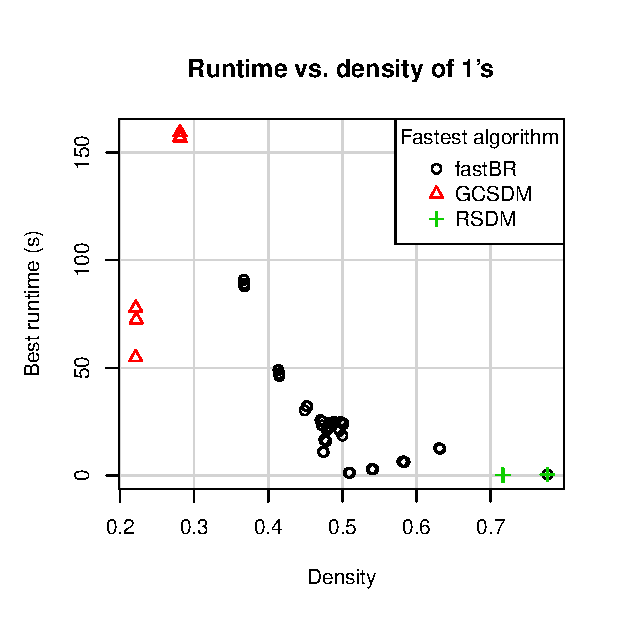
\includegraphics[height=8cm]{scatter_density.eps}
	    \end{center}
	\caption{Fastest algorithm runtime vs. density of 1's for all $SDMs$ under study.}
	\label{fig:scattDensity}
	\end{minipage}%
	~
	\begin{minipage}{.48\textwidth}
	    \begin{center}
	       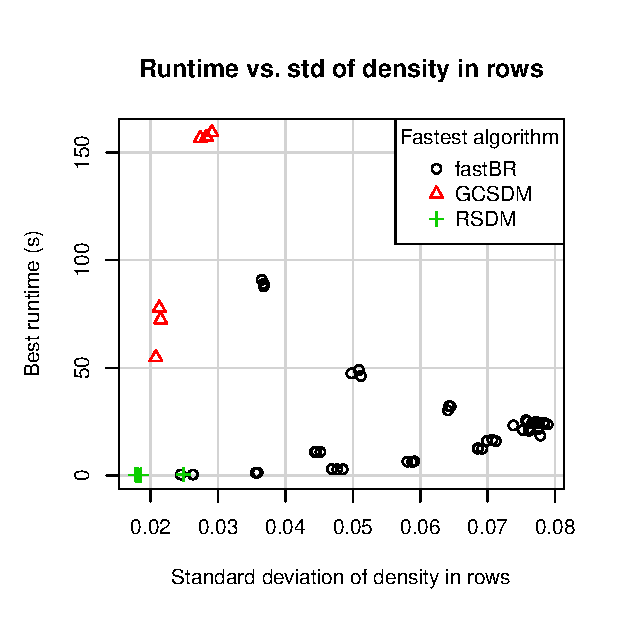
\includegraphics[height=8cm]{scatter_std.eps}
	    \end{center}
	\caption{Fastest algorithm runtime vs. standard deviation of density in rows for 
			 all $SDMs$ under study.}
	\label{fig:scattStd}
	\end{minipage}	
	\end{figure}	
	
	Since all matrices for this experiment have the same dimensions, we can say that low density
	matrices showed a relatively high complexity. For this reason, the apparent fact that GCSDM outperforms 
	the other algorithms for this kind of matrices, deserves special attention. On the other hand, the result 
	of RSDM on high density matrices seems less important. 
%	Figure~\ref{fig:scattDensity} shows a trend
%	to the reduction of the computational complexity of reduct computation regarding the increase of the
%	density in the $SDM$.
	
	Figure~\ref{fig:scattStd} shows a scatter graph of the runtime as a function of 
	the standard deviation of the density of 1's in the rows of the $SDM$. As it can be seen, there is no
	clear relationship between the runtime of the fastest algorithm and the standard deviation of density.
	Notice (combining information from Figures~\ref{fig:scattDensity} and~\ref{fig:scattStd}) that both, 
	low and high density matrices are related to low values of the standard deviation. In fact, it is not 
	possible to increase the standard deviation in the extreme values of density.
	
	Figure~\ref{fig:TimeReducts} shows a scatter graph of the runtime as a function of the 
	number of reducts in the $SDM$. There can be seen a positive correlation between these two variables.
	This is a natural trend, since the time complexity is at least as high as the space 
	complexity; which exceeds the size of the solution. For high density matrices, there are a low number
	of reducts which partially explains their lower computational cost (see Figure~\ref{fig:TimeReducts}). 
	
	\begin{figure}[htb]
	\begin{minipage}{.48\textwidth}
	    \begin{center}
	       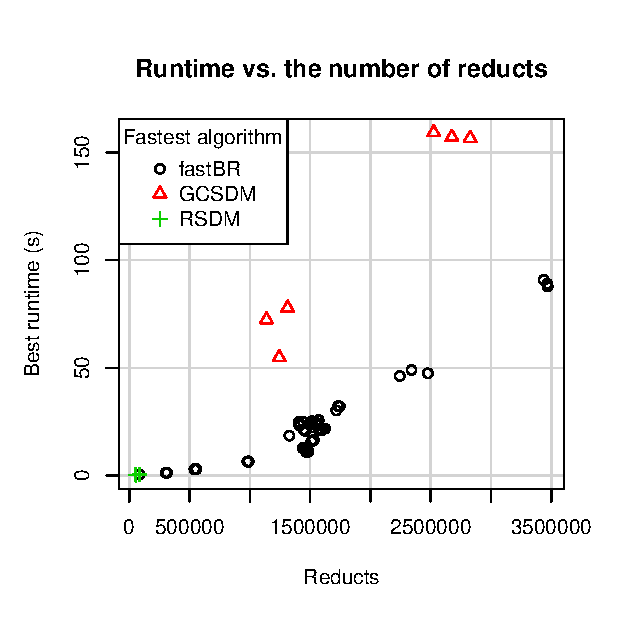
\includegraphics[height=8cm]{runtimeReducts.eps}
	    \end{center}
	\caption{Fastest algorithm runtime vs. the number of reducts.}
	\label{fig:TimeReducts}
	\end{minipage}%
	~
	\begin{minipage}{.48\textwidth}
	    \begin{center}
	       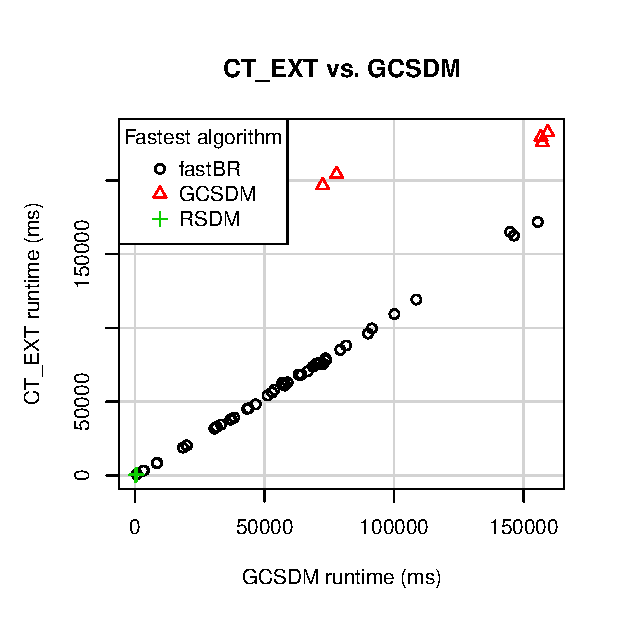
\includegraphics[height=8cm]{scatter_CTvsGAP.eps}
	    \end{center}
	\caption{CT\_EXT runtime vs. GCSDM runtime.}
	\label{fig:CTvsGAP}
	\end{minipage}	
	\end{figure}		
	
	Figure~\ref{fig:CTvsGAP} shows a scatter graph of the runtime of CT\_EXT vs. GCSDM for the $SDMs$ used in
	this experiment. Although GCSDM outperforms CT\_EXT in most cases. Based on the evidence of
	Figure~\ref{fig:CTvsGAP}, we proposed a one-sided t-test to evaluate the overall performance of GCSDM over
	CT\_EXT. Our \textbf{null hypothesis} is: \emph{there is no difference between the GCSDM and CT\_EXT runtime}.
	As \textbf{alternative hypothesis} we have: \emph{the runtime of CT\_EXT is higher than the runtime of GCSDM}.
	The output from the R software (Figure~\ref{fig:R_GCSDM}) supports the alternative hypothesis beyond a 95\%
	confidence interval. 
	
	\begin{figure}
		\qquad{}	Paired one-sided t-test\\

		data:  CT\_EXT runtime and GCSDM runtime\\
		t = 3.3, df = 56, p-value = 0.0008428\\
		alternative hypothesis: true difference in means is greater than 0\\
		95 percent confidence interval:\\
		 6976.147ms  \qquad{}  Inf\\
		sample estimates:\\
		mean of the differences \\
		 \qquad{}    14145.54ms
		 
		\centering
	  	\caption{R output for the t-test of mean CT\_EXT and GCSDM runtime.}
	  	\label{fig:R_GCSDM}
	\end{figure}
	
	In order to evaluate the performance improvement of GCSDM over fastBR, which is the fastest algorithm 
	reported in the literature, we present a new experiment. A total 	of 83 low density matrices, with 30 
	columns, was generated using the same procedure above described. This time, we generated $SDMs$ with 1000 
	rows. We evaluated the runtime of reduct computation over all matrices using fastBR and GCSDM. 
	Again we ran three execution of each possible combination in a randomized experiment.
	
	Figure~\ref{fig:runtime_low} shows the runtime as a function of the density of 1's in the $SDM$.
	There can be seen two interesting facts. First, there is a well defined
	line delimiting those $SDMs$ for which GCSDM is faster than fastBR (densities under 0.3). Second, the
	runtime of GCSDM increases monotonically with the increase of the density of 1's in the $SDM$.
	
	\begin{figure}[htb]
	\begin{minipage}{.48\textwidth}
	    \begin{center}
	       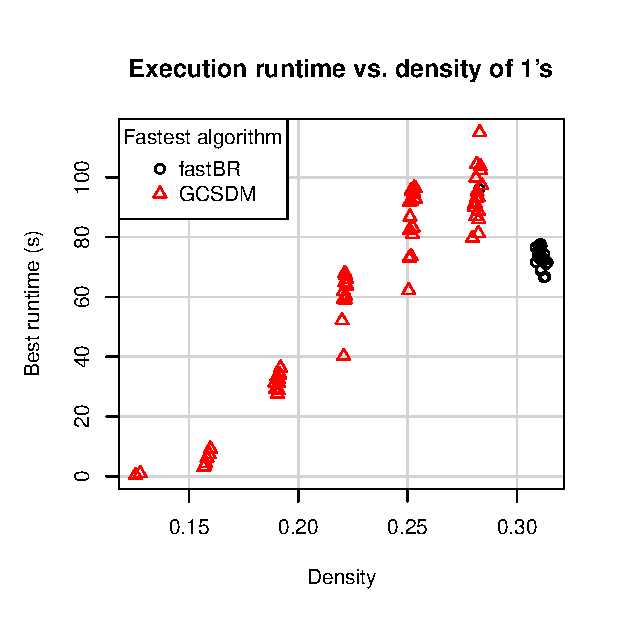
\includegraphics[height=8cm]{runtimeVSdensity_low.eps}
	    \end{center}
	\caption{Fastest algorithm runtime vs. density of 1's for all $SDMs$ under study.}
	\label{fig:runtime_low}
	\end{minipage}%
	~
	\begin{minipage}{.48\textwidth}
	    \begin{center}
	       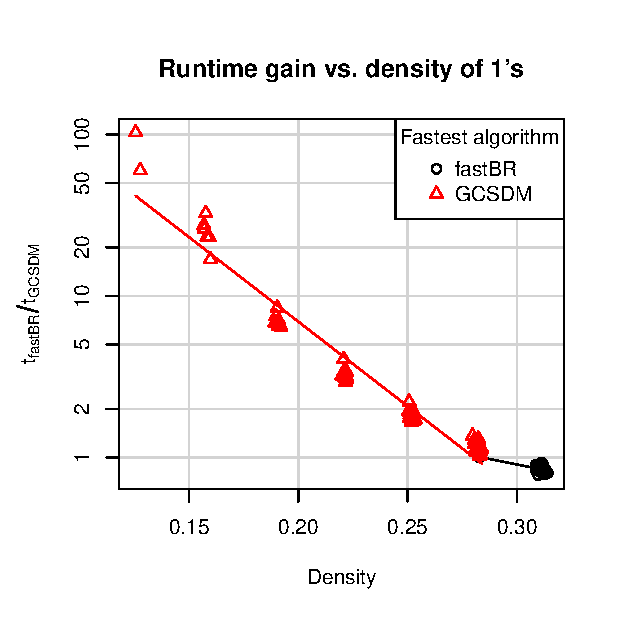
\includegraphics[height=8cm]{rate_runtime.eps}
	    \end{center}
	\caption{fastBR runtime over GCSDM runtime  vs. density of 1's for all $SDMs$ under study.}
	\label{fig:BRvsGAP}
	\end{minipage}	
	\end{figure}	
	
	In Figure~\ref{fig:BRvsGAP} we show the runtime rate between fastBR and GCSDM; where values above
	1 mean a runtime improvement of GCSDM over fastBR. For lower densities we have up to two orders of 
	magnitude rate.
	We found an exponential relationship between this rate and the density of the $SDM$. Notice that the 
	vertical axis in Figure~\ref{fig:BRvsGAP} is logarithmic.
	
	In order to explain this behaviour we must go deeply into the main difference between fastBR and GCSDM. 
	In GCSDM we compute the exclusion mask and evaluate the proposition~\ref{prop:exclude} only for those
	candidates proven as super-reducts, in order to verify them as reducts. In fastBR, on the other hand,
	the proposition~\ref{prop:exclude} is evaluated for each contributing candidate. As a result, fastBR
	evaluates less candidates than GCSDM but at a higher cost per candidate. The attribute exclusion
	occurs when there is at least one column, in the sub-matrix of $SDM$ formed by those attributes in the 
	current candidate, that can be removed without increasing the number of zero rows in this sub-matrix.
	The exclusion is more frequent in matrices with a higher density of 1's, as it can be inferred from  
	Figure~\ref{fig:BRvsGAP}. 
	
	Lets take for instance the extreme case of the identity matrix where there is no exclusion at all,
	since every attribute is indispensable to form a reduct. 	For this $SDM$, GCSDM needs to evaluate as 
	many candidates as fastBR but makes a single verification for exclusion with the set of all attributes. 
	On the other hand, fastBR verifies the exclusion for each candidate, which leads to a higher 
	computational cost.
	
	We used a one-sided t-test to evaluate the relative performance of GCSDM over fastBR in
	low density matrices. We selected the 62 $SDMs$ having a density 	of 1's lower than 0.3, from our original 
	83 matrices. As \textbf{null hypothesis} we have: \emph{there is no difference between the GCSDM and fastBR 
	runtime for $SDMs$ with density of 1's lower than 0.3}. As \textbf{alternative hypothesis} we have: 
	\emph{the runtime of fastBR is higher than the runtime of GCSDM for $SDMs$ with density of 1's lower than 
	0.3}. The following output from the R software (Figure~\ref{fig:R_fastBRvsGCSDM}) supports the alternative
	hypothesis beyond a 95\% confidence interval.
	
	\begin{figure}
		\qquad{}	Paired one-sided t-test\\

		data:  fastBR runtime and GCSDM runtime\\
		t = 11.0838, df = 61, p-value $<$ 2.2e-16\\
		alternative hypothesis: true difference in means is greater than 0\\
		95 percent confidence interval:\\
		 75124.33ms  \qquad{}  Inf\\
		sample estimates:\\
		mean of the differences \\
		 \qquad{}    88453.32ms
		 		 
		\centering
	  	\caption{R output for the t-test of mean fastBR and GCSDM runtime.}
	  	\label{fig:R_fastBRvsGCSDM}
	\end{figure}
	
\newpage 
\section{Conclusions}
	This PhD research proposal is focused on the problem of computing all the reducts and its related problem of
	computing shortest reducts of an information system. These are problems with exponential complexity which are
	actively studied. The theoretical bases were introduced to provide a unique nomenclature for the document and
	ensure that it is self contained. We present a revision of the related work to show the most relevant 
	approaches to the problem solution and based on this review we highlight the need for further research in this
	area. Then, the PhD research proposal is introduced; including justification and motivation, research 
	questions, our research objectives, and the methodology that will guide our research.
	
	As preliminary results, we we developed a hardware module for eliminating all non typical testors on the
	hardware component; reducing the amount of data that must be transferred to the PC and eliminating the final
	filtering. This hardware module is applicable to any algorithm for computing typical testors implemented on
	FPGA devices. This result was published in the memories of an international conference on reconfigurable
	computing.
	Our second preliminary result is a new hardware architecture of the CT EXT algorithm (which is one of the 
	most recent and fastest algorithms reported in the literature) for computing all the typical testors. Our 
	proposal traverses the search space in a different order than previous works, which evaluates less candidate 
	subsets than previous architectures, resulting in shorter runtime. This result has been reported in the 
	journal of Expert Systems With Applications. Additionally, we proposed two new algorithms for computing all 	
	the reducts, which are faster than existing algorithms for some kinds of datasets.
	RSDM was the fastest algorithm for $SDMs$ with density above 0.7 while GCSDM outperforms the rest of the
	evaluated algorithms in $SDMs$ with density under 0.3. These results will be reported in a congress or a 
	journal specialized in Rough Set Theory.

	Throughout our preliminary work, we covered most of the first four points in our proposed methodology, related
	to algorithms for computing all reducts of an information system.
	Finally, based on our preliminary results, we conclude that our objectives are reachable, in the scheduled
	time, following 	the proposed methodology.
	
%-------------------------------------------------------------------------------
% Bibliography
%-------------------------------------------------------------------------------
\newpage 
\bibliography{mybib}{}
\bibliographystyle{authordate1}
\end{document}
